\documentclass[twocolumn,11pt]{article}
\usepackage{graphicx}
\usepackage{amsmath}
\usepackage{xepersian}
\settextfont{IRXLotus}
\setlatintextfont[Scale=0.8]{Times New Roman}

\title{خلاصه های میان ترم یادگیری ماشین}
\author{امیر پورمند}
\begin{document}
\maketitle
\section{جلسه ۱}
تابع f همون تابعی هست که میخوایم یادبگیریم. 
goal یا g
خروجی الگوریتم ما هستش. 
$H$
همون مجموعه توابع هستش. میگن مدل یادگیری شامل دو چیزه
\begin{enumerate}
\item مجموعه فرضیه
\item الگوریتم یادگیری
\item تابع خطا
\end{enumerate}
سومی رو خودم اضافه کردم! چون به نظرم مهمه! 

الگوریتم یادگیری پرسپترون چیه؟
خب مشخصه مچموعه فرضیه اس توابع خطی ان. الگوریتم یادگیری اش
\begin{equation}
w(t+1) = w(t) + y_n x_n
\end{equation}
هست. تابع خطاش هم تعداد نقاط اشتباه کلاس بندی شده است! 
البته ما نقاط اشتباه کلاس بندی شده را با فرمول بالا اپدیت میکنیم. بهش میگن PLA . 

\section{جلسه ۲}
خب آیا واقعا یادگیری ممکنه؟
باید احتمالاتی به قضیه نگاه کنیم که بگیم بله. مسئله رو معادل مسئله تخمین گر میکنند که آیا تخمین گر میتونه با دقت خوبی اون پارامتر جمعیت رو مدل کنه یا نه؟

میگن بله میشه منتهی یه احتمالی داریم. احتمالش هم میشه همون باند هافدینگ و vc و بقیه علما. 

باند هافدینگ میگه احتمال این که دو تا تخمین و پارامتر از هم بیشتر از فلان مقدار فاصله داشته باشند چقدره؟

\begin{equation}
P(|\mu - \nu| > \epsilon) \leq 2 e^{-2 \epsilon^2 N}
\end{equation}
در واقع جمله بالا احتمالا درسته و مساوی اند
\lr{probably approximately correct} یا 
PAC

حالا چه ربطی به لرنینگ داشت؟ اون قرمز ها رو فرض بگیر تابع های غلط و اون سبز ها تابع های درست. میخوایم احتمال این رو حدس بزنیم که تابع ما درست باشه! 
و این احتماله با کم کردن باند زیاد میشه! اما اما این h عه یه تابع فیکسه و در واقع ما احتمال این که یک تابع فرضیه خوب باشه رو گفتیم. حالا تو یه روش خیلی ناشیانه میان میگن ما M
تا تابع توی فضای فرضیه داریم و هر کدوم ممکن هستند خوب باشند یا نباشند که باند هافدینگ تعمیم پیدا میکنه اینجوری و میشه

\begin{equation}
P(|E_{in}(h) - E_{out}(h)| > \epsilon) \leq 2 M e^{-2 \epsilon^2 N}
\end{equation}
راستی تعریف تابع ساین تو این درس خروجی منفی ۱ و مثبت ۱ داره. 

\section{جلسه سوم}
الگوریتم پاکت روی بهترین خطای سمپل خروجی برمیگردونه که بهتره! مثل پرسپترون معمولی فقط کانورج شده رو 
برنمیگردونه. 

جواب مسئله رگرسیون خطی یه جواب بسته اس به فرم
$w = (X^T X)^{-1} X^T y$

\clearpage
\section{جلسه چهارم}
فرمول خطای in-sample

\begin{equation}
E_{in}(h) = \frac{1}{N} \sum_{n=1}^N
 e(h(x_n),f(x_n)) 
 \end{equation}
 
 خطای out-of-sample
\begin{equation}
E_{out}(h) = E_x[e(h(x),f(x)]
\end{equation}

در اینجا دو تا مفهوم معادل قدیم داریم که به
 \lr{False Positive}
  میگن 
 \lr{False Accept}
 و به 
 \lr{False Negative}
میگن 
\lr{False Reject}
و تو مثال های مختلف معمولا یکی مهم تره! 

تابع هدف ما همیشه میتونه تابع نباشه! یعنی به ازای دو تا ورودی عین هم خروجی مختلف داشته باشه! 
در این حالت ما 
$f(x) = E[y|x]$
بدست میاریم!

خب تا حالا میدونیم که یادگیری امکان پذیره. چرا؟ چون به احتمال زیاد که فرمول داره داریم
$E_{in}(h) \simeq E_{out}(h)$
و البته داریم
$E_{in}(h) \simeq 0$

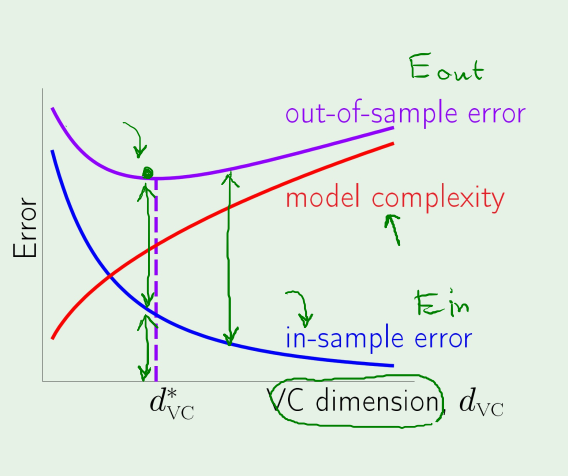
\includegraphics[scale=0.5]{vc-error.png} 

\section{جلسه پنجم}
مفهوم دایکاتمی Dichotomy اینه که اگر n تا نقطه داشته باشیم چند تا برچسب دهی مختلف داریم که فضای فرضیه ما بتونه تولیدش کنه! دی که میدونی معنی دو میده. دایکاتمی یعنی تقسیم به دو بخش. چند حالت میشه تقسیم به دو قسمت کرد. 

بهش میگن فرضیه کوچک. اگر تعداد توابع فضای حالت بی نهایت هم باشه تعداد دایکاتمی ها میشه ۲ به توان تعداد نقاط حداکثر! 

تعداد حداکثر دایکاتمی ها تو یک فضای مشخص میشه
$m_H(N)$
.
به این تابع رشد هم میگن. 
این تابع خیلی جالبه یا بریک پوینت داریم که میشه چندجمله ای و خیلی هم مشخصه فرمش یا بریک پوینت نداریم و میشه ۲ به توان N.


پس اگر بتونیم بجای M همون m را بذاریم خیلی خوب میشه! 
شرطش اینه که تابع m چند جمله ای باشه فقط که ثابت میشه اگر بریک پوینت داشته باشه چند جمله ای هست و یه فرم 
مشخصی هم داره. 

بریک پوینت یه مفهوم گره خورده با بعد vc هست. میگن که اگر بتونیم هر دیتاست از سایز N رو با فضای فرضیه مون دو قسمت کنیم اینجا یعنی بعد vc ما حداقل N عه. ماکزیمم تعداد نقاطی که میشه کامل shatter کرد رو میگن بعد VC. 
و یکی بیشتر بعد 
VC
میشه بریک پوینت که هست
$k_{breakpoint} = d_{vc} - 1$

پس تعریف بریک پوینت میشه حداقل تعداد نقاطی که نتوان همه حالاتش رو shatter کرد. 

\section{جلسه ششم}
دو تا اثبات داریم یکی این که اگر بریک پوینت داشته باشیم 
$m_H(N)$
چند جمله ای هست. 

یکی دیگه این که میشه به جای M
بزرگ گذاشت m.

به یه فرمولی میرسیم که داریم:

\begin{equation}
m_H(N) \leq B(N,K) \leq \sum_{i=0}^{k-1} {N \choose k}  
\leq N^{k-1} = N^d
\end{equation}
که میگن B یعنی تعداد دایکاتمی ها وقتی n
 تا نقطه و بریک پوینت k رو داریم. 


البته با جایگذاری فرمول کمی فرق میکنه و باند وی سی به شکل زیر بدست میاد:

\begin{equation}
P(|E_{in}(h) - E_{out}(h)| > \epsilon) \leq
4 m_H(2N) e^{-\frac{1}{8} \epsilon^2 N}  
\end{equation}

\section{جلسه هفتم}
خب ما باید بتونیم بعد VC
رو اثبات کنیم. برای این دو طرف معادله باید ثابت بشه. 
یک: وجود داره یه روش خاصی برای n نقاط که همه حالاتش رو بشه 
shatter کرد. 
این یعنی 
$d_{vc} \geq N$

دو: هیچ حالتی از N+1 نقطه رو نمیشه 
shatter کرد!

\begin{equation}
P(|E_{in}(h) - E_{out}(h)| > \epsilon) \leq
4 m_H(2N) e^{-\frac{1}{8} \epsilon^2 N} \simeq 
N^d e^{-N}
\end{equation}

که از این نتیجه میگیریم به عنوان یک قاعده که N
باید حداقل ۱۰ برابر بعد VC
باشه که مسئله 
generalize 
شه. 

\begin{gather}
\delta = 4 m_H(2N) e^{-\frac{1}{8} \epsilon^2 N} \\
\epsilon = \sqrt{\frac{8}{N} ln\frac{4m_H(N)}{\delta}}
\end{gather}

که در نظر بگیر که دلتا احتمال اتفاق بد هست. و رابطه خودمون رو هم کلا به این صورت مینویسیم

\begin{equation}
E_{out}(h) \leq E_{in}(h) + \delta
\end{equation}

\section{جلسه هشتم}
ببین یه تریدآف داریم هر چه تابع پیچیده تر باشه تخمین یا 
approximation
بهتره و هر چی تابع ساده تر باشه
generalization 
بهتره. باند بایاس واریانس میخوایم بدست بیاریم منتهی دو تا مسئله هست یک تابع خطا هست 
که MSE هست و دو مسئله هست که باید رگرسیون باشد. 

خب میرسیم به فرمول بایاس واریانس:
\begin{equation}
\begin{split}
E_D[(g^{(D)}(x) - f(x))^2] &= \\
E_D[g^{(D)}(x) - \bar{g}(x))^2] &+\\ (\bar{g}(x)- f(x))^2
\end{split}
\end{equation}

یک درس مهم اینه که پیچیدگی مدل برابر هست با پیچیدگی دیتا نه لزوما پیچیدگی تابع! 

\section{جلسه نهم}
نگاه کردن به داده قبل از درست کردن مدل ممکنه باعث بشه یه جستجویی تو ذهن ما شکل بگیره و یه سری مدل ها محدود بشه به خاطر همین جستجو که بهش میگیم
\lr{data snooping}

برای رگرسیون logistic نیاز به سیگموید داریم چون خاصیت زیر را دارد و برامون مهمه!

\begin{equation}
S(x) = \frac{1}{1+e^{-x}} = 
\frac{e^x}{1+e^x} = 1-S(-x)
\end{equation}

مدل ما در اینجا یک مدل خطیه
\begin{equation}
g(x) = \theta(w^T x) 
\end{equation}

خطای ما باید حساب بشود
\begin{equation}
P(y|x) = 
\begin{cases}
h(x), &y=1 \\
1-h(x), &y=-1
\end{cases} = 
\theta(y w^T x) 
\end{equation}
و بعد با روش MLE
خطا رو بصورت زیر بدست میاریم:

\begin{equation}
E_{in}(w) = \frac{1}{N} \sum_{n=1}^N 
ln(1+e^ {-y_n w^T x_n}) 
\end{equation}
که به این خطا خطای کراس انتروپی میگیم.

الگوریتم یادگیری مون هم باشه مینیمایز کردن همین تابع که با روش گرادیان کاهشی پیش میریم به امید خدا.

پس در هر مرحله گرادیان کل داده ها را بدست میاریم و میریم جلو
\begin{equation}
w(t+1) = w(t) - \eta \nabla E_{in}(w(t))
\end{equation}

پس سه تا روش خطی یاد گرفتیم:
یکی پرسپترون برای مسئله کلاس بندی که با خطای کلاس بندی پیش میره و الگوریتم یادگیری اش PLA
و Pocket 
هست
 و دیگری رگرسیون که با خطای MSE
پیش میره و الگوریتم یادگیری اش
\lr{pseudo-inverse}
است
و دیگری رگرسیون لاچیستیک که با خطای کراس انتروپی پیش میره
و الگوریتم یادگیری اش گرادیان کاهشی!

\section{جلسه دهم}
خب روش ما تا حالا GD بوده و بهتر است از گرادیان تصادفی استفاده کنیم که گرادیان بردار وزن یک داده است. 

الگوریتم بک پروپگیشن و شبکه عصبی رو از جای دیگه ای باید بخونم خوب نگفته. 
\section{جلسه یازدهم}

حتی اگر بدونیم که تابع ما مثلا درجه ۱۰ هست و داده کافی نداشته باشیم نباید تابع درجه ۱۰ فیت کنیم زیرا نویز را یاد میگیرد و overfit میشود! 

حالا نویز تصادفی و نویز قطعی چی هستند؟
یه مساله ای رو در نظر بگیریم که به یه دیتایی مدل مرتبه ۱۰ و مرتبه ۲ فیت کنیم. مشخصه که 
$E_{out}$
هر کدوم بیشتر باشه بدتره. میایم خطای out-of-sample 
مرتبه ۱۰ رو منهای ۲ میکنیم. 

میبینیم که دو تا عامل تاثیر دارن روی این که این معیار منفی یا مثبت بشه. یکی نویز تصادفی هست که همون نویزی هست که تو دیتا بوده و دیگری نویز قطعی که با نشون دهنده پیچیدگی مدله. 

حالا فهمیدن وقتی تعداد دیتا کمه تقریبا همیشه مرتبه ۲ بهتره و هیچ لولی از نویز تصادفی رو نمیتونه تحمل کنه و اگر تعداد دیتا زیاد باشه کم کم تحمل مدل نسبت به نویز تصادفی زیاد میشه که البته با 
$\sigma^2$ 
نشونش میدن و همین جور رابطه ای رو هم کما بیش با نویز قطعی فهمیدن. 

نویز قطعی رو میگن قسمتی از تابع اصلی که فرضیه ما نمیتونه کپچر کنه و در واقع انقدری پیچیده نیست که بتونه بفهمه. 
تفاوت اصلی اش با نویز تصادفی اینه که به فضای فرضیه بستگی داره. بعضی علما میگن معادل بایاس هست نویز قطعی. 

حالا که فهمیدیم اصل قضیه overfitting 
مال نویزه و نویزها رو هم شناختیم میرسیم به داستان راه حل که علما میگن دو تا روش هست

\begin{enumerate}
\item Validation
\item Regularization
\end{enumerate}

\section{روابط مهم}
\begin{gather}
4 m_H(2N) e^{-\frac{1}{8}\epsilon^2 N} \leq \delta \\
\epsilon \leq \sqrt{\frac{8}{N}\ln{\frac{4m_{\mathcal{H}}(2N)}{\delta}}}
\\
N \geq \frac{8}{\epsilon^2}\ln{\frac{4m_{\mathcal{H}}(2N)}{\delta}}
\\
N \geq \frac{8}{\epsilon^2}\ln{\frac{4(2N)^{d_{vc}}}{\delta}}
\end{gather}
\end{document}